%; whizzy paragraph -pdf xpdf -latex ./whizzypdfptex.sh
%; whizzy-paragraph "^\\\\begin{frame}"
% latex beamer presentation.
% platex, latex-beamer でコンパイルすることを想定。 

%     Tokyo Debian Meeting resources
%     Copyright (C) 2011 Junichi Uekawa
%     Copyright (C) 2011 Nobuhiro Iwamatsu

%     This program is free software; you can redistribute it and/or modify
%     it under the terms of the GNU General Public License as published by
%     the Free Software Foundation; either version 2 of the License, or
%     (at your option) any later version.

%     This program is distributed in the hope that it will be useful,
%     but WITHOUT ANY WARRANTY; without even the implied warreanty of
%     MERCHANTABILITY or FITNESS FOR A PARTICULAR PURPOSE.  See the
%     GNU General Public License for more details.

%     You should have received a copy of the GNU General Public License
%     along with this program; if not, write to the Free Software
%     Foundation, Inc., 51 Franklin St, Fifth Floor, Boston, MA  02110-1301 USA

\documentclass[cjk,dvipdfmx,12pt]{beamer}
\usetheme{Tokyo}
\usepackage{monthlypresentation}

%  preview (shell-command (concat "evince " (replace-regexp-in-string "tex$" "pdf"(buffer-file-name)) "&")) 
%  presentation (shell-command (concat "xpdf -fullscreen " (replace-regexp-in-string "tex$" "pdf"(buffer-file-name)) "&"))
%  presentation (shell-command (concat "evince " (replace-regexp-in-string "tex$" "pdf"(buffer-file-name)) "&"))

%http://www.naney.org/diki/dk/hyperref.html
%日本語EUC系環境の時
\AtBeginDvi{\special{pdf:tounicode EUC-UCS2}}
%シフトJIS系環境の時
%\AtBeginDvi{\special{pdf:tounicode 90ms-RKSJ-UCS2}}

\title{東京エリアDebian勉強会}
\subtitle{第81回 2011年10月度}
\author{前田 耕平 mkouhei@debian.or.jp\\IRC nick: mkouhei}
\date{2011年10月22日}
\logo{
\includegraphics[width=8cm]{image200607/openlogo-light.eps}}

\begin{document}

\frame{\titlepage{}}


\begin{frame}{設営準備にご協力ください。}
宴会場所を誰か探してください。\\
※昨年の反省を踏まえ、つくば駅前限定で。
\end{frame}


\section{}
\begin{frame}
 \frametitle{Agenda}
\begin{minipage}[t]{0.45\hsize}
  \begin{itemize}
  \item 注意事項
	\begin{itemize}
	 \item 飲酒禁止
	 \item 宗教禁止
	 \item 営利活動禁止
	\end{itemize}
   \item 最近あったDebian関連のイベント報告
	\begin{itemize}
        \item 第80回 東京エリアDebian勉強会
	 \item Debian温泉2011
	\end{itemize}
 \end{itemize}
\end{minipage} 
\begin{minipage}[t]{0.45\hsize}
 \begin{itemize}
   \item Debian Trivia Quiz
   \item 事前課題紹介
   \item Debianとはなにか?
   \item HaskellとDebianの辛くて甘い関係
   \item 快適な \LaTeX 環境あります
   \item レポートPDFの自動生成
   \item 月刊debhelper 第1回
  \end{itemize}
\end{minipage}
\end{frame}

\begin{frame}
 \frametitle{前回}
\begin{minipage}[t]{0.45\hsize}
  \begin{itemize}
  \item 注意事項
	\begin{itemize}
	 \item 飲食禁止
	 \item 宗教禁止
	 \item 営利活動禁止
	\end{itemize}
  \end{itemize}
\end{minipage}
\begin{minipage}[t]{0.45\hsize}
 \begin{itemize}
  \item 最近あったDebian関連のイベント報告
    \begin{itemize}
    \item 第80回 東京エリアDebian勉強会
    \item Debian 温泉 2011
    \end{itemize}
 \end{itemize}
\end{minipage}
\end{frame}


\emtext{イベント報告}

\emtext{Debian 温泉 2011}

\begin{frame}{開催場所}
\begin{minipage}{0.6\hsize}
\begin{itemize}
\item 開催場所は 伊東
\item 9/19(土)15時に現地集合
\item 熱海からの伊東線が30分に1本しかないので通勤ラッシュなみに混んでた
\item 駅前商店街と旅館以外に特に何もなく、三連休初日だというのに街は閑散としてた
\item 今回の参加者は8名
\end{itemize}
\end{minipage}
\begin{minipage}{0.35\hsize}
%\includegraphics[width=1.4\hsize]{image201110/ito-onsen-map.jpg}
\end{minipage}
\end{frame}

\begin{frame}{会場}

会場は、伊東駅から徒歩10分くらいの山喜温泉旅館。
\begin{center}
%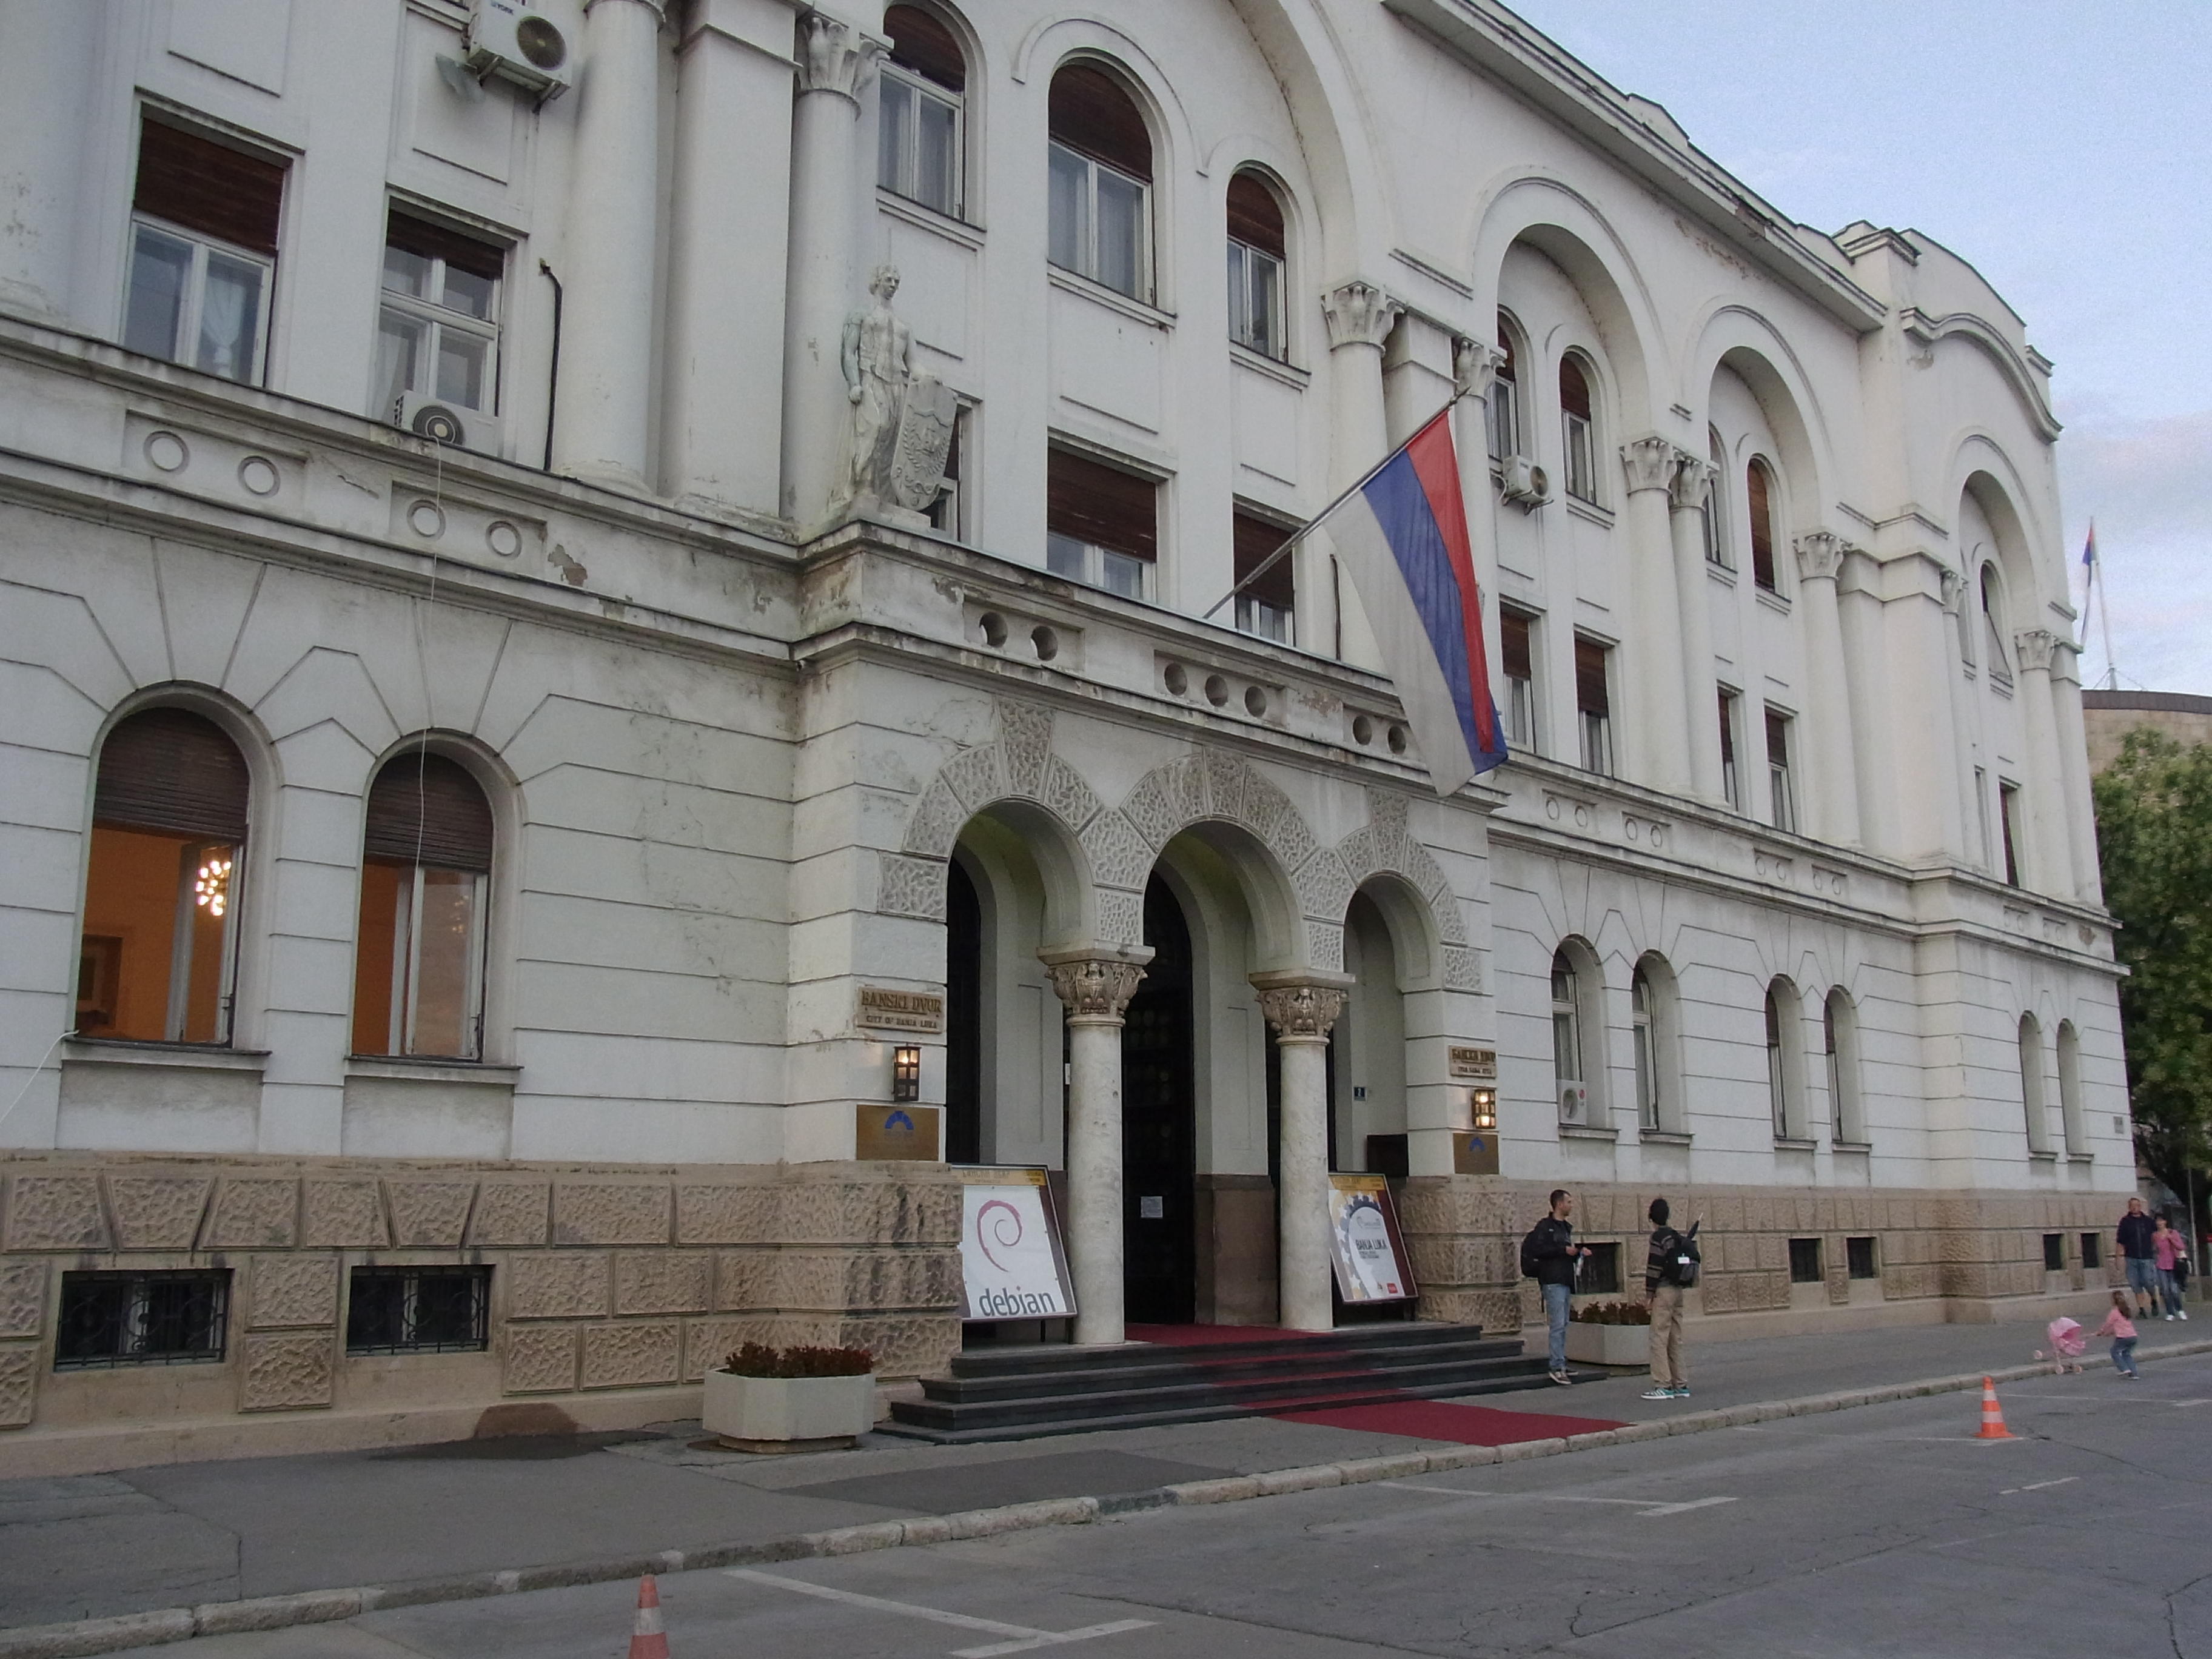
\includegraphics[width=0.8\hsize]{image201108/debconf11_venue1.jpg}
\end{center}
\end{frame}

\begin{frame}{オレオレHacklab}

オレオレHacklab はハック専用の部屋。\\
朝5時前までハックしてました
\begin{center}
%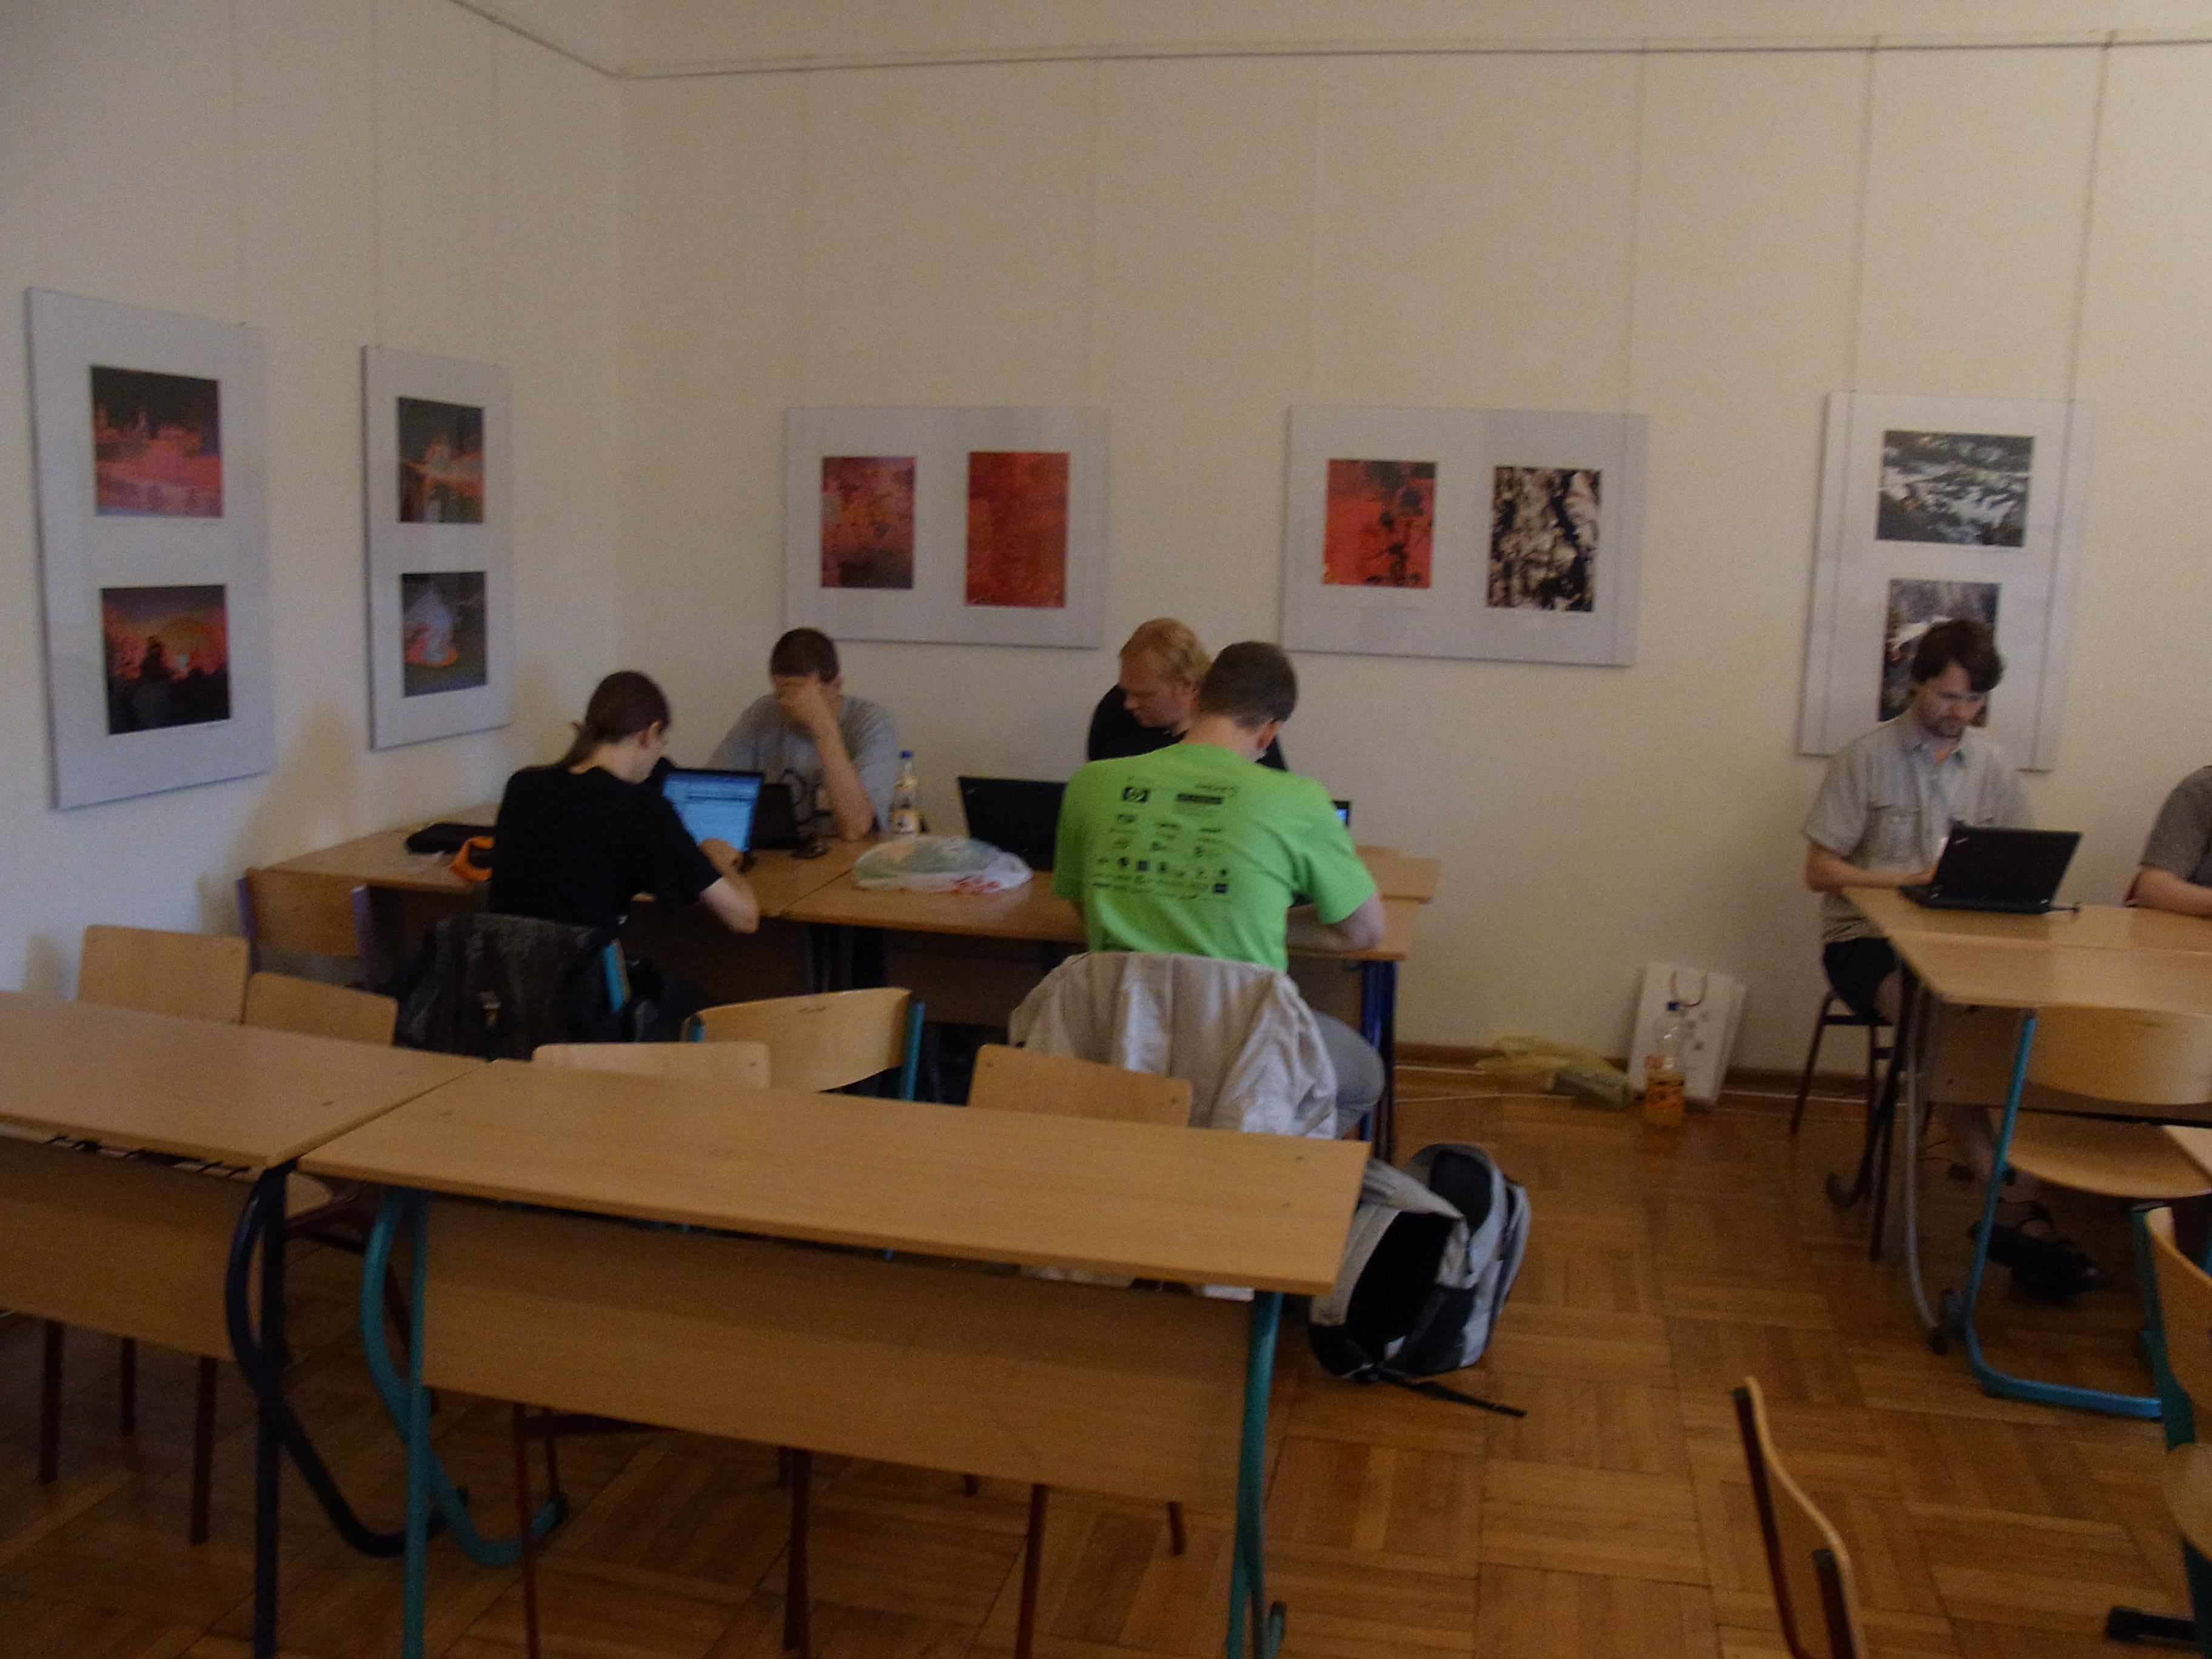
\includegraphics[width=0.8\hsize]{image201108/debconf11_hacklab1.jpg}
\end{center}
\end{frame}

\begin{frame}{スケジュール}

\begin{itemize}
\item 15時に集合
\item 18時までの夕食までそれぞれハック
\item 19時から21時まで会議室を借りてハックや、Mini DebConfに向けたディスカッション
\item 21時から翌朝5時頃までガンバルマン大会
\item 6時半-7時頃起床し、温泉で朝風呂
\item 7時半から朝食、その後解散
\end{itemize}
\end{frame}

\begin{frame}{次回のDebian温泉}

次回のDebian温泉もやりたい人が企画&計画&実行しる。

\end{frame}

\emtext{DWN quiz}

\section{DWN quiz}
\begin{frame}{Debian 常識クイズ}

Debian の常識、もちろん知ってますよね?
知らないなんて恥ずかしくて、知らないとは言えないあんなことやこんなこと、
みんなで確認してみましょう。

今回の出題範囲は\url{debian-devel-announce@lists.debian.org} に投稿された
内容とDebian Project Newsなどからです。

\end{frame}

\subsection{問題}
%; whizzy-master ../debianmeetingresume201101.tex
% 以上の設定をしているため、このファイルで M-x whizzytex すると、whizzytexが利用できます。
%
% ちなみに、クイズは別ブランチで作成し、のちにマージします。逆にマージし
% ないようにしましょう。
% (shell-command "git checkout quiz-prepare")

\santaku
{Debian温泉2011の1日目はいつでしょうか?}
{9/17}
{9/18}
{9/19}
{A}
{さっきの話を聞いていればわかって当然ですね}

\santaku
{8月にDebianは誕生日を迎えました。何周年でしたでしょうか?}
{17}
{18}
{19}
{B}
{今年もお祝いしましたよね}

\santaku
{最新のDebian Newsはいつ発行されたでしょうか?}
{9/17}
{9/18}
{9/19}
{C}
{購読していれば知っていて当然ですね}

\santaku
{10/17の''delegation for the DSA team''で代表団に任命されなかったのは誰でしょう?}
{Faidon Liambotis}
{Luca Filipozzi}
{Nobuhiro Iwamatsu}
{C}
{他に任命されたのは、の全部で合計名です。}

\santaku
{Wheezyフリーズの予定はいつでしょう?}
{2012年4月}
{2012年6月}
{2012年8月}
{B}
{あと6ヶ月ですよ!}

\santaku
{1.16.1がリリースされたdpkgに該当するのはどれ?}
{\texttt{dpkg-buildpackage}コマンドでは \texttt{CFLAGS, CXXFLAGS, LDFLAGS, CPPFLAGS, FFLAGS}の\texttt{export}が必須になった}
{\texttt{dpkg-deb}コマンドに\texttt{--verbose}オプションが追加された}
{Multi-Archフィールドがサポートされた}
{B}
{\texttt{dpkg-buildpackage}ではこれらのオプションが不要になりました。Multi-Archは1.16.2からサポートされる予定です。\texttt{dpkg-deb -x/--extract -v/--verbose}で\texttt{dpkg-deb -X/--xextract}と同じ動きをするようになりました。}



\emtext{prework}

{\footnotesize
 \begin{prework}{ koedoyoshida }

\begin{multicols}{2}
\begin{enumerate}
{\tiny
\item 仕事はさておくとして、自宅環境ではサーバ系はDebian、クライアント系はWindowsにしています。サーバにはXも入れていないのでGUI系操作はすべてWindowsということになります。クライアントでやっていることがDebianで出来るかですが...
  \begin{itemize}
{\tiny
  \item メール:Beckey:以前(Thunderbird 2.X)移行を検討したけれど振り分けルール(日本語(である/でない)のメール判別、複合条件のand/or,fromおよび宛先(to/cc/bcc)判別)が複雑でTBで再現ができず移行困難で断念
  \item ブラウザ:メインブラウザがOpera:速度面でFirefox(iceweasel)より快適。サブはFirefoxとChromeなのでiceweaselとChromiumに移行するのはもっさりすること以外は特に問題なし
  \item エディタ:秀丸:Emacsへ移行すれば問題なし
  \item デバイスコントロール:
    \begin{itemize}
{\tiny
    \item X Video Station:TV録画サーバ:対応ソフトウェアがWinowsXPのみ、アナログ放送が終了したのでお役御免かと思いきや、xvproxy(\footnote{\url{http://xvproxy.local.io/c5/}})とデジアナ変換で寿命が延びた。Garapon TV等へ移行予定。動作監視(EPGチェック)はDebianにて実施中
    \item Garapon TV:ワンセグ録画サーバ:Firefoxで閲覧しているのでiceweaselへ移行可能。動作監視(ハングチェック等、異常時自動再起動)についてはDebianにて実施中
    \item Scansnap:自炊PDFを管理:移行可能らしいが詳細未調査
    \item iPhone\&iPod:音楽および動画ライブラリ:移行可能らしいが詳細未調査
}
    \end{itemize}
}
  \end{itemize}
}
\end{enumerate}
\end{multicols}
\end{prework}

\begin{prework}{ sheeta38 }

\begin{enumerate}
\item 授業(プログラミング入門1)のレポート作成。 gccと \LaTeX を用いている
\item プログラミング、およびLinuxにもっと触れる。現状、コンピュータに関して知っていることがあまりに少ないと感じており、これらに触れていくことで、少しずつ肩をならしていきたい。

C言語も\LaTeX、あるいは他の言語(Ruby, Python等)も、Windowsで環境を整えようとすれば可能だ。ただしLinuxの方が環境構築が容易であると思う。
他に具体的なLinux(Debian)の利点があるならば知りたい。
\end{enumerate}

\end{prework}

\begin{prework}{ r.matsumiya@syntaxerror.biz }

開発メイン、レポート作成。両方ともDebian使ってます。
\end{prework}

\begin{prework}{ 吉野(yy\_y\_ja\_jp) }

某社製オフィススイートのファイルをレイアウトを壊さず表示・編集したいです。

\end{prework}

\begin{prework}{ キタハラ }

時間ギリギリなので、将来やりたいことで、Linuxだと
やりにくそうなものをあげてみる。(よい方法があれば教えてください。)
\begin{enumerate}
\item 地デジの録画 \\
色々方法があるようですが、コンテンツ保護とかで面倒そう
\item 自炊コンテンツの作成\\
スキャンはできそうだが、OCRとかスキャナ付属のおまけに負けて、Windowsを使いそうな気が……。
\end{enumerate}

\end{prework}

\begin{prework}{ 木村 陽一 }

DebianでApache+SQLite+PHPなWebアプリ開発をしています。そろそろC\#やVB.NETもやりたいと思っていますが、MonoのVB.NETコンパイラは不安定で機能が十分でないのでWindows環境をVMに用意して開発しようと思っています。
\end{prework}

\begin{prework}{ dictoss(杉本 典充) }

\begin{itemize}
\item web閲覧、メール、プログラム開発は仕事も自宅もDebian GNU/Linuxで行っている
\item MIDIキーボード練習はWindowsをひとまず使っている。(Linuxでもできると思うがあまり調べていないため)
\item ビデオ録画(PT2を使用)はFreeBSDで行っている。自宅webサーバがFreeBSDだったので、それに相乗りする形でそのまま使い続けているから
\end{itemize}

\end{prework}

\begin{prework}{ Kiwamu Okabe }

Haskell!Debianが最も適しています!

\end{prework}

\begin{prework}{ 田原悠西 }

コンピュータを使ってやりたいことであり、やっていることは仕事とかインターネットを使ったりとか。Debianを使ってできています。

\end{prework}

\begin{prework}{ Arnaud Fontaine }

I'm a Debian developer who arrived in Tokyo last year and interested in meeting up some other developers. I'm using Debian only at work and home.

\end{prework}

\begin{prework}{ Hirotaka Kawata }

\begin{enumerate}
\item 趣味で Python で簡単なプログラムの作成や、アセンブラ(binutils)やコンパイラ(gcc)の新しいアーキテクチャへの移植。仕事で PHP, Rails や HTML, CSS をつかった Web プログラムの作成。遊びでゲームとか(フライトシミュレータなど)
\item できる
\end{enumerate}

\end{prework}

\begin{prework}{ mitty }

ファイル等のバックアップや重複管理をもっと楽にしたい。

普段使いのPCとは別に、ファイルサーバ(NAS)としてUbuntuを用いているが、バックアップや世代化、ダウンロードしてきたisoイメージなどのファイル重複チェックなど、ほとんど適宜手動でやっているため、ある程度自動化出来ると嬉しい。
\end{prework}

\begin{prework}{ osamu@debian.org }

Debian文書の整理(DDPのXETEX対応)、内容更新 ー 使用理由: 自明

実際は私物の写真の編集・整理ぐらいがDEBIAN「利用目的」です。 ー 他のプラットフォームはすぐ消えていくが、いつも最新システムでいられるしコンンパティビリティーの心配がない。なんと言ってもお金がかからない。こんな所が理由です。

正直なところ、ブラウザーを使う以外は意外とDEBIANを使っていません。Debianは少々荒削りですが、使いやすいのと、今までの習慣で使っています。最初は日本語サポートできるがベースが英語というのが理由でしたが、いまとなってはUBUNTUをなぜ使わないかとなります。まあ、あえていえば自分たちで作っているという気がするのが理由ですかね。
\end{prework}

\begin{prework}{ pi8027 }

\begin{enumerate}
\item \begin{itemize}
\item プログラム、証明、文書などの作成
\item 講義のノートを取る作業、レポートを作成する作業
\item 情報収集
\item 自分自身に関わる色々な物事の管理(予定管理とか)
\item これらの作業の部分的もしくは完全な自動化
\end{itemize}
\item できます
\end{enumerate}

\end{prework}

\begin{prework}{ taitioooo(長谷川) }

家のKVMやXenserverを管理できるセルフポータル整備しようとしています。Linuxでできますが、debianでできません。Centos使ってます。

\end{prework}

\begin{prework}{ 野島 貴英 }

\begin{enumerate}
\item \begin{enumerate}
\item 自分独自仕様のクールなGUIとクールな入出力デバイスを持つクールなPC/モバイル機を作って人に自慢する
\item とにもかくにもクールな爆安PC/モバイル機を作って社会的/経済的に厳しいところでとにかく流行らせる。コンテンツ作らせる。お金まわす
\end{enumerate}
\item いや、その。Debian(Linux)以外だとかなり難易度高いっすよね?\\
※中年になってから、厨二病患ってます...
\end{enumerate}
\end{prework}

\begin{prework}{ tai@rakugaki.org }

\begin{center}
{\tiny
\begin{tabular}{|l|c|c|l|}
\hline
& 有無 & 使ってるか & 備考 \\
\hline
ウェブ利用 &○&△& CLIから一発検索したりは便利 \\
メール &○&×& ウェブベースに流れ中 \\
その他ネット利用 &△&△& バックアップ環境で使うことが \\
ソフト開発 &○&△& 商用系の環境が動かない \\
日記,ログ &○&○& \\
文書作成 &○&○& \\
図面作成 &△&×& 商用系アプリが動かない \\
デモ,プレゼン &△&△& 一部の便利ツールがない \\
ストリーミング &△&△& \\
\hline
\end{tabular}
}
\end{center}
{\tiny
基盤はDebian、入出力フロントエンドはWindowsで分担利用。
普段は
\begin{commandline}
 Windows(画面転送用)
 -> Windows on Debian(デスクトップ環境)
 -> Debian over ssh/HTTP/CIFS/...(HOME+作業環境)
\end{commandline}
と入れ子環境で生活してる。あと自作単機能端末やアプライアンスは全部Debian。むしろ他を選ぶ理由がない。

Debian(Linux)を使ってない分野は、全部Xが絡む部分…
OSXに行く人の気持ち、よくわかります。でもCLI/サーバ環境は
Debianがベストなので今の分担構成。あと、CLIベースで
作っておくとssh+screen/tmuxでどこからでも環境再現できるので
そこは便利。emacsで大体なんでも動くし(便利とはいい難いものもあるが...)。

閲覧系はiPhone/Androidを使ってる時間がどんどん増えているので、Debian(Linux)というよりPC系環境がま
あ全敗していきそう。AndroidはAndroid(Linux)だからLinux勝利か、というとまた微妙な感じではある。
}
\end{prework}


\begin{prework}{ 岩松 信洋 }
  \begin{itemize}
  \item やりたいこと
  \begin{enumerate}
  \item DVCam を使った Debianでの Ustream 配信。
  昔はできたんですけどね。サウンド周りを直していません。
  \item 完全自動クロスコンパイル環境の構築。今は一部のパッケージを
  ネイティブでコンパイルされている必要があるので。
  \end{enumerate}
  \item やっていること
  \begin{enumerate}
  \item いつでも、どこでも、誰とでも Debian を使っています。
  \item インターネットを見るのもDebianだし、開発環境もDebianです。
  \end{enumerate}
  \end{itemize}
\end{prework}



\begin{prework}{ まえだこうへい }

  \begin{enumerate}
  \item やりたいことは、自分や家族の生活を便利にすること
  \item こまめ監視カメラなど、部分的には出来ているけど、まだ完全ではない。今の勤務先もCentOSやUbuntuで、Debianは使ってない。前者は技術的(ハードウェア)やリソース(要は自分の時間と金)の問題、後者は政治的、人的な理由
  \end{enumerate}
  Debianだけな生活を送るために、頑張るのです。
\end{prework}


}

\emtext{Debianとはなにか?}
\emtext{HaskellとDebianの辛くて甘い関係}
\emtext{快適な \LaTeX 環境あります}
\emtext{レポートPDFの自動生成}
\emtext{月刊debhelper 第1回}

\emtext{今後のイベント}

\begin{frame}{今後のイベント}
 
\begin{itemize}
 \item 10月度HackCaff
 \item 11月 OSC 2011 Tokyo/Fall
 \item 11-12月 第1回 Debian Users勉強会(仮)
 \item 12月 第82回 東京エリアDebian勉強会

\end{itemize}
\end{frame}

\begin{frame}{今日の宴会場所}

つくば駅前のどこか。
\end{frame}

\end{document}

;;; Local Variables: ***
;;; outline-regexp: "\\([ 	]*\\\\\\(documentstyle\\|documentclass\\|emtext\\|section\\|begin{frame}\\)\\*?[ 	]*[[{]\\|[]+\\)" ***
;;; End: ***
